% !TEX program = xelatex
\documentclass[a4paper]{article}
\usepackage[utf8]{inputenc}
\usepackage{amsmath}
\usepackage{graphicx}
\usepackage{fontspec}
\usepackage{ctex}
\usepackage{hyperref}
\usepackage{listings}
\usepackage{color}

\usepackage[margin=1in]{geometry}

\setmainfont{Times New Roman}
\setmonofont{Noto Sans Mono}

\setCJKmainfont{WenQuanYi Micro Hei}
\setCJKsansfont{WenQuanYi Micro Hei}
\setCJKmonofont{WenQuanYi Micro Hei Mono}

\lstdefinestyle{minijava}{
    language=Java,
    basicstyle=\ttfamily,
    keywordstyle=\color{blue}\ttfamily,
    stringstyle=\color{red}\ttfamily,
    commentstyle=\color{green}\ttfamily,
    numberstyle=\color{magenta}\ttfamily,
    breaklines=true
}

\lstdefinestyle{llvm}{
    basicstyle=\ttfamily,
    breaklines=true
}

\title{编译Project报告}
\author{14307130245 张剑锋}

\begin{document}
\maketitle

本项目实现了MiniJava语言的编译器前、后端。项目使用JFlex、Bison实现了源码到AST的转换,
并利用ASM和LLVM等库生成JVM字节码和LLVM中间表示以及本地代码。

\section{原理}
\subsection{词法分析}
词法分析是把输入文件的字符流解析成token流的过程。
一般情况下,编译器会对所有合法token构建一个DFA来实现线性时间的解析过程。
主流的Lexer均使用正则表达式生成DFA的实现。
本项目选用JFlex。主要原因是JFlex语法接近flex,使我相当于同时掌握了flex的用法。
同时,JFlex可以与Bison很好地配合工作。

\subsection{句法分析}
句法分析以token流为输入,输出语法树。不同的生成工具会产生不同的解析算法,
比如ANTLR、JavaCC会产生LL的解析器,而Bison、Yacc、CUP产生LALR的解析器。
本项目使用Bison。选用Bison的主要原因是Bison生成LR系列的解析器;我以前有使用LL解析器的经验,
因此这次项目想尝试不同的选择。另一方面的原因是Bison在开源软件中非常流行。

\section{源码结构}
{\tt src/main/java/taiho/minijava}目录下是主要的源码文件。其中:
\begin{itemize}
    \item {\tt Lexer.l}是词法文件,用以生成{\tt Lexer.java}
    \item {\tt Parser.y}是语法文件,用以生成{\tt Parser.java};
          此外还可以生成LALR解析器的状态表文件{\tt Parser.output}
    \item {\tt Position.java}是用以描述token在源码中的位置的类
    \item {\tt Analyzer.kt}是用以进行语义分析的类,用途包括分析类成员、方法参数和局部变量,
        解析符号和表达式类型
    \item {\tt Main.kt}是命令行程序入口
\end{itemize} \par
{\tt src/main/java/taiho/minijava/ast}目录下是AST的节点类。 \par
{\tt src/main/java/taiho/minijava/backend}目录下是后端的实现。其中:
\begin{itemize}
    \item {\tt astprinter}是AST输出类
    \item {\tt interpreter}是解释器
    \item {\tt bytecode}是JVM字节码生成
    \item {\tt llvm}是LLVM IR和本地代码生成
\end{itemize}
其它文件是测试文件。

\section{错误修复}
运行{\tt java -jar build/libs/MiniJaba-all.jar -i samples/errors.java}
可以看见示例的含有错误的源文件是如何输出错误信息的:

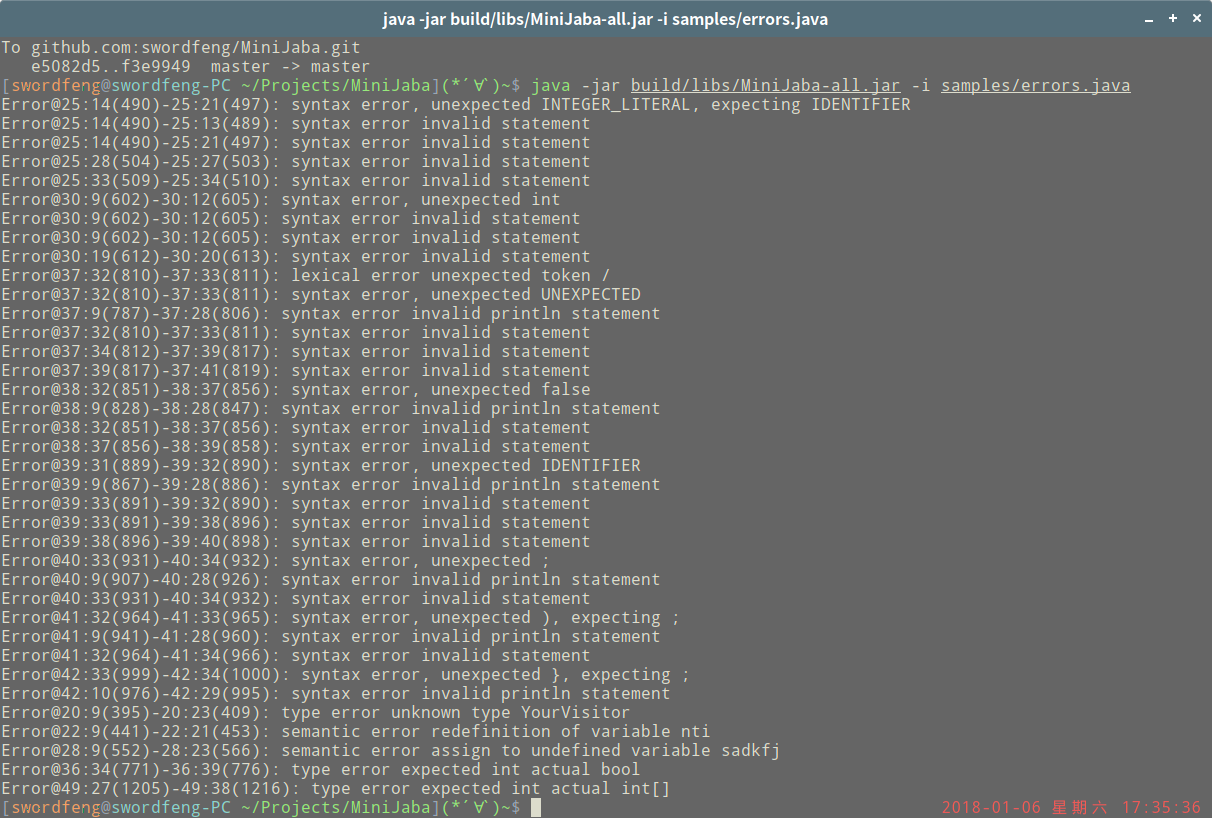
\includegraphics[width=\textwidth]{screenshot}

\subsection{词法错误}
{\tt errors.java}第37行:
\begin{lstlisting}[style=minijava]
    System.out.println(100 / false);
\end{lstlisting} \par
Lexer遇到无法匹配字符,输出:{\tt Error@37:32(810)-37:33(811): lexical error unexpected token /}

\subsection{语法错误}
语法错误的处理相比非常复杂。可以看出示例中有大量语法错误,但是错误仅仅报告了非法的语句。
在Bison中,当发生错误时,解析器会尝试在当前栈上放上一个特殊的{\bf error} token。
如果当前没有规则移入一个{\bf error},解析器会丢弃栈上最后一个符号并再次尝试,
直到找到一个能够放入{\bf error}的位置。放入{\bf error}后,
解析器会丢弃当前位置之后的符号直到存在下一个符号对应的规则。
这就导致了如果错误处理规则存在疏漏,就容易发生{\bf error}“吃掉”附近过多token的情况。
而严密的错误处理规则会导致句法文件中存在比正常规则更多的错误处理规则。
因此在本项目中,为了使代码简洁,只处理了在一个语句中发生了错误的情况。
一旦错误发生,这个错误所在位置附近的语句会在语法树中被处理成一个非法语句节点,来防止它影响其它语句的解析。

简单的语法错误,如第30行:
\begin{lstlisting}[style=minijava]
    int sadkfj;
\end{lstlisting} \par
该错误在于在一个语句后面出现了一个声明。可以看到对应的错误信息:
{\tt Error@30:9(602)-30:12(605): syntax error, unexpected int}

\subsection{语义错误}
本项目处理了几类简单的语义错误。
\subsubsection{类型错误}
\begin{lstlisting}[style=minijava]
    System.out.println(100 + false);
\end{lstlisting} \par
输出:{\tt Error@36:34(771)-36:39(776): type error expected int actual bool}
\subsubsection{符号未定义}
\begin{lstlisting}[style=minijava]
    sadkfj = 2333;
\end{lstlisting} \par
输出:{\tt Error@28:9(552)-28:23(566): semantic error assign to undefined variable sadkfj}
\subsubsection{符号重定义}
\begin{lstlisting}[style=minijava]
    int nti;
    boolean nti;
\end{lstlisting} \par
输出:{\tt Error@22:9(441)-22:21(453): semantic error redefinition of variable nti}
\par
语义分析对所有类先进行一次遍历,分析类型和类成员的符号定义和它们的作用域;再对所有方法进行一次遍历,
先分析参数和本地变量的定义,再解析所有语句内的符号。

\section{额外功能}
本项目主要添加的额外功能是一个解释器和两个编译器的后端实现。

\subsection{解释器}
解释器直接在JVM上实现。对于Int,Bool和IntArray类型直接使用对应的JVM类型;
对于Object,解释器实现了一个Obj类,用以记录对象的类、父对象和成员变量。
所有的成员变量实现在每个Obj内的HashMap里。

解释器运行过程中也会动态检查变量使用时的类型和声明是否一致,不一致会抛出异常退出。

\subsection{字节码编译器}
JVM方法执行的时候,有两个本地内存空间:局部变量表和操作数栈。

数值计算的时候,把两个数值推入操作数栈,执行计算指令,计算指令会弹出两个数值,算得结果推回栈上。
JVM里没有直接对Bool类型的操作;所有的Bool被编译为byte,在运算时是当作int处理的。

对象方法调用的时候,把对象、方法参数按顺序推到栈上,然后调用对应的方法。由于Java中所有方法调用
基本都是虚方法调用,因此本项目中所有方法调用都是使用invokevirtual指令。

对于被调用方法,所有的参数一开始都被放在局部变量表里。返回时把返回值放在栈上,根据对应类型执行返回指令。

所有对象在创建的时候都必须调用构造方法,构造方法有个特殊的名字<init>。
该项目对所有MiniJava类实现了默认构造方法,调用时使用invokespecial指令。

JVM运行过程中,变量的类型是动态的:虚拟机没有保证变量表或操作数栈上一个值的类型。
不过字节码里对于类成员的类型都有静态定义。如果调用时类型不一致会引发虚拟机异常。

\subsection{本地代码编译器}
本地代码编译器没有直接生成本地代码指令,而是生成LLVM IR再用LLVM提用的方法生成本地代码。

MiniJava和LLVM的类型如下对应:
\begin{itemize}
    \item Bool \Rightarrow{} i1
    \item Int \Rightarrow{} i32
    \item IntArray \Rightarrow{} i32*
    \item Object \Rightarrow{} 对应类型的type的指针
\end{itemize}

为了处理动态分发,对于所有的MiniJava类,项目生成如下的结构
\begin{lstlisting}[style=llvm]
    type { base_struct, fields... }
\end{lstlisting} \par
对于继承其它类的类来说,base\_struct是基类结构;对于无继承的类来说,base\_struct是如下的虚表指针:
\begin{lstlisting}[style=llvm]
    { i8** }*
\end{lstlisting} \par
这样就保证了所有对象的开头位置指向它的虚表。

虚表是一个指针数组,每一个成员方法对应一项。子类中的方法若和父类方法有相同名字,
则这个方法在虚表中的位置和父类方法位置相同。这样就能实现运行时的动态分发。

数组类型用简单的方式处理:分配数组时比请求大小多一个int,分配到的内存空间第一个int的内容为数组长度,
从第二个位置开始才是真正的数组内容。

LLVM IR中,所有变量的值是不可变的。可变状态需要用alloc指令分配内存空间;实际代码中这个空间分配在栈上。
堆空间可以用malloc指令分配。

本项目中所有的虚表生成的符号为“类名\$\$”,所有方法生成的符号为“类名\$方法名”。
方法的第一个参数是this指针,其后是原方法的参数依次排列。方法的局部变量都用alloc分配在栈上。
新数组和新对象都用memset初始化为0;随后数组被写入长度,对象被写入虚表指针。

\end{document}
